\documentclass[twoside]{book}

% Packages required by doxygen
\usepackage{fixltx2e}
\usepackage{calc}
\usepackage{doxygen}
\usepackage[export]{adjustbox} % also loads graphicx
\usepackage{graphicx}
\usepackage[utf8]{inputenc}
\usepackage{makeidx}
\usepackage{multicol}
\usepackage{multirow}
\PassOptionsToPackage{warn}{textcomp}
\usepackage{textcomp}
\usepackage[nointegrals]{wasysym}
\usepackage[table]{xcolor}

% Font selection
\usepackage[T1]{fontenc}
\usepackage[scaled=.90]{helvet}
\usepackage{courier}
\usepackage{amssymb}
\usepackage{sectsty}
\renewcommand{\familydefault}{\sfdefault}
\allsectionsfont{%
  \fontseries{bc}\selectfont%
  \color{darkgray}%
}
\renewcommand{\DoxyLabelFont}{%
  \fontseries{bc}\selectfont%
  \color{darkgray}%
}
\newcommand{\+}{\discretionary{\mbox{\scriptsize$\hookleftarrow$}}{}{}}

% Page & text layout
\usepackage{geometry}
\geometry{%
  a4paper,%
  top=2.5cm,%
  bottom=2.5cm,%
  left=2.5cm,%
  right=2.5cm%
}
\tolerance=750
\hfuzz=15pt
\hbadness=750
\setlength{\emergencystretch}{15pt}
\setlength{\parindent}{0cm}
\setlength{\parskip}{3ex plus 2ex minus 2ex}
\makeatletter
\renewcommand{\paragraph}{%
  \@startsection{paragraph}{4}{0ex}{-1.0ex}{1.0ex}{%
    \normalfont\normalsize\bfseries\SS@parafont%
  }%
}
\renewcommand{\subparagraph}{%
  \@startsection{subparagraph}{5}{0ex}{-1.0ex}{1.0ex}{%
    \normalfont\normalsize\bfseries\SS@subparafont%
  }%
}
\makeatother

% Headers & footers
\usepackage{fancyhdr}
\pagestyle{fancyplain}
\fancyhead[LE]{\fancyplain{}{\bfseries\thepage}}
\fancyhead[CE]{\fancyplain{}{}}
\fancyhead[RE]{\fancyplain{}{\bfseries\leftmark}}
\fancyhead[LO]{\fancyplain{}{\bfseries\rightmark}}
\fancyhead[CO]{\fancyplain{}{}}
\fancyhead[RO]{\fancyplain{}{\bfseries\thepage}}
\fancyfoot[LE]{\fancyplain{}{}}
\fancyfoot[CE]{\fancyplain{}{}}
\fancyfoot[RE]{\fancyplain{}{\bfseries\scriptsize Generated by Doxygen }}
\fancyfoot[LO]{\fancyplain{}{\bfseries\scriptsize Generated by Doxygen }}
\fancyfoot[CO]{\fancyplain{}{}}
\fancyfoot[RO]{\fancyplain{}{}}
\renewcommand{\footrulewidth}{0.4pt}
\renewcommand{\chaptermark}[1]{%
  \markboth{#1}{}%
}
\renewcommand{\sectionmark}[1]{%
  \markright{\thesection\ #1}%
}

% Indices & bibliography
\usepackage{natbib}
\usepackage[titles]{tocloft}
\setcounter{tocdepth}{3}
\setcounter{secnumdepth}{5}
\makeindex

% Hyperlinks (required, but should be loaded last)
\usepackage{ifpdf}
\ifpdf
  \usepackage[pdftex,pagebackref=true]{hyperref}
\else
  \usepackage[ps2pdf,pagebackref=true]{hyperref}
\fi
\hypersetup{%
  colorlinks=true,%
  linkcolor=blue,%
  citecolor=blue,%
  unicode%
}

% Custom commands
\newcommand{\clearemptydoublepage}{%
  \newpage{\pagestyle{empty}\cleardoublepage}%
}

\usepackage{caption}
\captionsetup{labelsep=space,justification=centering,font={bf},singlelinecheck=off,skip=4pt,position=top}

%===== C O N T E N T S =====

\begin{document}

% Titlepage & ToC
\hypersetup{pageanchor=false,
             bookmarksnumbered=true,
             pdfencoding=unicode
            }
\pagenumbering{alph}
\begin{titlepage}
\vspace*{7cm}
\begin{center}%
{\Large S\+C\+A\+RA Robotics }\\
\vspace*{1cm}
{\large Generated by Doxygen 1.8.13}\\
\end{center}
\end{titlepage}
\clearemptydoublepage
\pagenumbering{roman}
\tableofcontents
\clearemptydoublepage
\pagenumbering{arabic}
\hypersetup{pageanchor=true}

%--- Begin generated contents ---
\chapter{Namespace Index}
\section{Namespace List}
Here is a list of all documented namespaces with brief descriptions\+:\begin{DoxyCompactList}
\item\contentsline{section}{\hyperlink{namespaceanimation__ex}{animation\+\_\+ex} }{\pageref{namespaceanimation__ex}}{}
\end{DoxyCompactList}

\chapter{Hierarchical Index}
\section{Class Hierarchy}
This inheritance list is sorted roughly, but not completely, alphabetically\+:\begin{DoxyCompactList}
\item \contentsline{section}{inverse\+\_\+kinematics.\+S\+C\+A\+R\+A\+\_\+\+IK}{\pageref{classinverse__kinematics_1_1_s_c_a_r_a___i_k}}{}
\item Enum\begin{DoxyCompactList}
\item \contentsline{section}{inverse\+\_\+kinematics.\+method\+IK}{\pageref{classinverse__kinematics_1_1method_i_k}}{}
\end{DoxyCompactList}
\end{DoxyCompactList}

\chapter{Class Index}
\section{Class List}
Here are the classes, structs, unions and interfaces with brief descriptions\+:\begin{DoxyCompactList}
\item\contentsline{section}{\hyperlink{classinverse__kinematics_1_1method_i_k}{inverse\+\_\+kinematics.\+method\+IK} }{\pageref{classinverse__kinematics_1_1method_i_k}}{}
\item\contentsline{section}{\hyperlink{classinverse__kinematics_1_1_s_c_a_r_a___i_k}{inverse\+\_\+kinematics.\+S\+C\+A\+R\+A\+\_\+\+IK} }{\pageref{classinverse__kinematics_1_1_s_c_a_r_a___i_k}}{}
\end{DoxyCompactList}

\chapter{Namespace Documentation}
\hypertarget{namespaceanimation__ex}{}\section{animation\+\_\+ex Namespace Reference}
\label{namespaceanimation__ex}\index{animation\+\_\+ex@{animation\+\_\+ex}}
\subsection*{Functions}
\begin{DoxyCompactItemize}
\item 
\mbox{\Hypertarget{namespaceanimation__ex_a1bc3cd0fd2deafcc870466428b5cb0d6}\label{namespaceanimation__ex_a1bc3cd0fd2deafcc870466428b5cb0d6}} 
def {\bfseries update\+\_\+line} (num, data, line)
\end{DoxyCompactItemize}
\subsection*{Variables}
\begin{DoxyCompactItemize}
\item 
\mbox{\Hypertarget{namespaceanimation__ex_a02d5ed3cc605cf0681febc2b37bae780}\label{namespaceanimation__ex_a02d5ed3cc605cf0681febc2b37bae780}} 
{\bfseries fig1} = plt.\+figure()
\item 
\mbox{\Hypertarget{namespaceanimation__ex_a7a011d85142c64a3467c3a1f2d196ef9}\label{namespaceanimation__ex_a7a011d85142c64a3467c3a1f2d196ef9}} 
{\bfseries data} = np.\+random.\+rand(2, 25)
\item 
{\bfseries line\+\_\+ani}
\item 
\mbox{\Hypertarget{namespaceanimation__ex_a76edff2bd76ff7bcc36dfb40ccb284cf}\label{namespaceanimation__ex_a76edff2bd76ff7bcc36dfb40ccb284cf}} 
{\bfseries fig2} = plt.\+figure()
\item 
\mbox{\Hypertarget{namespaceanimation__ex_a17e317a806a8c4ddea11d6f1ac831201}\label{namespaceanimation__ex_a17e317a806a8c4ddea11d6f1ac831201}} 
{\bfseries x} = np.\+arange(-\/9, 10)
\item 
\mbox{\Hypertarget{namespaceanimation__ex_ae4a2b3f3de462924cd1035084da069e7}\label{namespaceanimation__ex_ae4a2b3f3de462924cd1035084da069e7}} 
{\bfseries y} = np.\+arange(-\/9, 10).reshape(-\/1, 1)
\item 
\mbox{\Hypertarget{namespaceanimation__ex_a634b973c81c0506526ec7e541414d60c}\label{namespaceanimation__ex_a634b973c81c0506526ec7e541414d60c}} 
{\bfseries base} = np.\+hypot(x, y)
\item 
\mbox{\Hypertarget{namespaceanimation__ex_af37231c6533d6c9e51f943bb5045a3bd}\label{namespaceanimation__ex_af37231c6533d6c9e51f943bb5045a3bd}} 
list {\bfseries ims} = \mbox{[}$\,$\mbox{]}
\item 
{\bfseries im\+\_\+ani}
\item 
\mbox{\Hypertarget{namespaceanimation__ex_a3b7f94a8144cc8d7d9a0a72539056411}\label{namespaceanimation__ex_a3b7f94a8144cc8d7d9a0a72539056411}} 
{\bfseries metadata}
\end{DoxyCompactItemize}


\subsection{Detailed Description}
\begin{DoxyVerb}=========================
Simple animation examples
=========================

This example contains two animations. The first is a random walk plot. The
second is an image animation.
\end{DoxyVerb}
 

\subsection{Variable Documentation}
\mbox{\Hypertarget{namespaceanimation__ex_ab0383e2a36c5426861a44c34ab3fcc59}\label{namespaceanimation__ex_ab0383e2a36c5426861a44c34ab3fcc59}} 
\index{animation\+\_\+ex@{animation\+\_\+ex}!im\+\_\+ani@{im\+\_\+ani}}
\index{im\+\_\+ani@{im\+\_\+ani}!animation\+\_\+ex@{animation\+\_\+ex}}
\subsubsection{\texorpdfstring{im\+\_\+ani}{im\_ani}}
{\footnotesize\ttfamily animation\+\_\+ex.\+im\+\_\+ani}

{\bfseries Initial value\+:}
\begin{DoxyCode}
1 =  animation.ArtistAnimation(fig2, ims, interval=50, repeat\_delay=0,
2                                    blit=\textcolor{keyword}{True})
\end{DoxyCode}
\mbox{\Hypertarget{namespaceanimation__ex_a9106489832e7ffd8ba98df3ba6d206b4}\label{namespaceanimation__ex_a9106489832e7ffd8ba98df3ba6d206b4}} 
\index{animation\+\_\+ex@{animation\+\_\+ex}!line\+\_\+ani@{line\+\_\+ani}}
\index{line\+\_\+ani@{line\+\_\+ani}!animation\+\_\+ex@{animation\+\_\+ex}}
\subsubsection{\texorpdfstring{line\+\_\+ani}{line\_ani}}
{\footnotesize\ttfamily animation\+\_\+ex.\+line\+\_\+ani}

{\bfseries Initial value\+:}
\begin{DoxyCode}
1 =  animation.FuncAnimation(fig1, update\_line, 25, fargs=(data, l),
2                                    interval=50, blit=\textcolor{keyword}{True})
\end{DoxyCode}

\chapter{Class Documentation}
\hypertarget{classinverse__kinematics_1_1method_i_k}{}\section{inverse\+\_\+kinematics.\+method\+IK Class Reference}
\label{classinverse__kinematics_1_1method_i_k}\index{inverse\+\_\+kinematics.\+method\+IK@{inverse\+\_\+kinematics.\+method\+IK}}


Inheritance diagram for inverse\+\_\+kinematics.\+method\+IK\+:
\nopagebreak
\begin{figure}[H]
\begin{center}
\leavevmode
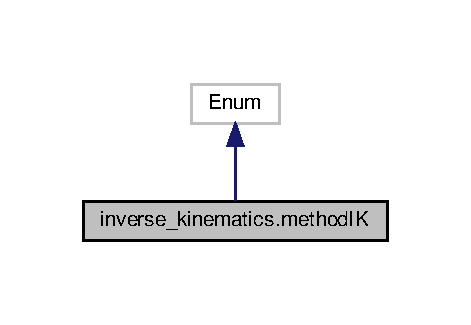
\includegraphics[width=226pt]{classinverse__kinematics_1_1method_i_k__inherit__graph}
\end{center}
\end{figure}


Collaboration diagram for inverse\+\_\+kinematics.\+method\+IK\+:
\nopagebreak
\begin{figure}[H]
\begin{center}
\leavevmode
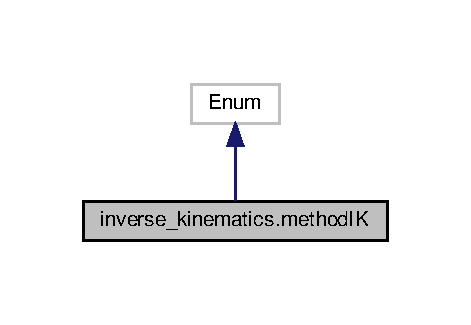
\includegraphics[width=226pt]{classinverse__kinematics_1_1method_i_k__coll__graph}
\end{center}
\end{figure}
\subsection*{Static Public Attributes}
\begin{DoxyCompactItemize}
\item 
\mbox{\Hypertarget{classinverse__kinematics_1_1method_i_k_accf053233216234c1aefcb94554bd148}\label{classinverse__kinematics_1_1method_i_k_accf053233216234c1aefcb94554bd148}} 
int {\bfseries J\+A\+C\+O\+B\+I\+A\+N\+\_\+\+PS} = 0
\item 
\mbox{\Hypertarget{classinverse__kinematics_1_1method_i_k_a705e9e4236af7884c98ff566c16dec2b}\label{classinverse__kinematics_1_1method_i_k_a705e9e4236af7884c98ff566c16dec2b}} 
int {\bfseries F\+A\+B\+R\+IK} = 1
\item 
\mbox{\Hypertarget{classinverse__kinematics_1_1method_i_k_a74977b66ae013de67710ee80b806cc52}\label{classinverse__kinematics_1_1method_i_k_a74977b66ae013de67710ee80b806cc52}} 
int {\bfseries J\+A\+C\+O\+B\+I\+A\+N\+\_\+\+I\+NV} = 2
\end{DoxyCompactItemize}


The documentation for this class was generated from the following file\+:\begin{DoxyCompactItemize}
\item 
src/\+Sim/inverse\+\_\+kinematics.\+py\end{DoxyCompactItemize}

\hypertarget{classinverse__kinematics_1_1_s_c_a_r_a___i_k}{}\section{inverse\+\_\+kinematics.\+S\+C\+A\+R\+A\+\_\+\+IK Class Reference}
\label{classinverse__kinematics_1_1_s_c_a_r_a___i_k}\index{inverse\+\_\+kinematics.\+S\+C\+A\+R\+A\+\_\+\+IK@{inverse\+\_\+kinematics.\+S\+C\+A\+R\+A\+\_\+\+IK}}
\subsection*{Public Member Functions}
\begin{DoxyCompactItemize}
\item 
def \hyperlink{classinverse__kinematics_1_1_s_c_a_r_a___i_k_a68c331184cb5d0b9bc28567922cedd01}{\+\_\+\+\_\+init\+\_\+\+\_\+} (self, joint\+\_\+len)
\item 
def \hyperlink{classinverse__kinematics_1_1_s_c_a_r_a___i_k_ac5dd573c899961b0b402ecab76c34499}{plan\+\_\+path} (self, delta=0.\+1)
\item 
\mbox{\Hypertarget{classinverse__kinematics_1_1_s_c_a_r_a___i_k_aaeb154dd436a588ef5363b71402bfbea}\label{classinverse__kinematics_1_1_s_c_a_r_a___i_k_aaeb154dd436a588ef5363b71402bfbea}} 
def {\bfseries set\+\_\+target} (self, x, y)
\item 
\mbox{\Hypertarget{classinverse__kinematics_1_1_s_c_a_r_a___i_k_aa94976c8e18b7c591c5df10adaa0aeb2}\label{classinverse__kinematics_1_1_s_c_a_r_a___i_k_aa94976c8e18b7c591c5df10adaa0aeb2}} 
def {\bfseries linear\+\_\+spline} (self, last, first, step\+\_\+size)
\item 
\mbox{\Hypertarget{classinverse__kinematics_1_1_s_c_a_r_a___i_k_afa9572a2aea8af0d0fbb72bc002e08d4}\label{classinverse__kinematics_1_1_s_c_a_r_a___i_k_afa9572a2aea8af0d0fbb72bc002e08d4}} 
def {\bfseries jacobian\+\_\+inverse\+\_\+method} (self)
\item 
\mbox{\Hypertarget{classinverse__kinematics_1_1_s_c_a_r_a___i_k_a7ee747d7965af2222bfee3f208ef9228}\label{classinverse__kinematics_1_1_s_c_a_r_a___i_k_a7ee747d7965af2222bfee3f208ef9228}} 
def {\bfseries jacobian\+\_\+pseudoinverse\+\_\+method} (self)
\item 
\mbox{\Hypertarget{classinverse__kinematics_1_1_s_c_a_r_a___i_k_aa382d8317262aedf27231f6376a08f2b}\label{classinverse__kinematics_1_1_s_c_a_r_a___i_k_aa382d8317262aedf27231f6376a08f2b}} 
def {\bfseries calc\+\_\+joint\+\_\+pos} (self)
\item 
\mbox{\Hypertarget{classinverse__kinematics_1_1_s_c_a_r_a___i_k_a778650d0d211dd62191b0709c7a57e43}\label{classinverse__kinematics_1_1_s_c_a_r_a___i_k_a778650d0d211dd62191b0709c7a57e43}} 
def {\bfseries F\+A\+B\+R\+I\+K\+\_\+method} (self)
\item 
\mbox{\Hypertarget{classinverse__kinematics_1_1_s_c_a_r_a___i_k_aa0472b7a8858db808c4bd50147dd7d9b}\label{classinverse__kinematics_1_1_s_c_a_r_a___i_k_aa0472b7a8858db808c4bd50147dd7d9b}} 
def {\bfseries check\+\_\+position\+\_\+viability} (self)
\item 
\mbox{\Hypertarget{classinverse__kinematics_1_1_s_c_a_r_a___i_k_a2ac203c33ebd9b611c6a0501ef1c35c1}\label{classinverse__kinematics_1_1_s_c_a_r_a___i_k_a2ac203c33ebd9b611c6a0501ef1c35c1}} 
def {\bfseries effector\+\_\+pos} (self)
\item 
\mbox{\Hypertarget{classinverse__kinematics_1_1_s_c_a_r_a___i_k_a1fa1b3d3ddb59508945708457908f9ff}\label{classinverse__kinematics_1_1_s_c_a_r_a___i_k_a1fa1b3d3ddb59508945708457908f9ff}} 
def {\bfseries run} (self)
\item 
\mbox{\Hypertarget{classinverse__kinematics_1_1_s_c_a_r_a___i_k_a667f32f399dff864418aee0b18d20f55}\label{classinverse__kinematics_1_1_s_c_a_r_a___i_k_a667f32f399dff864418aee0b18d20f55}} 
def {\bfseries draw} (self)
\item 
\mbox{\Hypertarget{classinverse__kinematics_1_1_s_c_a_r_a___i_k_ac990ff34f4db55c1806fe4a980ee7f31}\label{classinverse__kinematics_1_1_s_c_a_r_a___i_k_ac990ff34f4db55c1806fe4a980ee7f31}} 
def {\bfseries calc\+\_\+angles} (self)
\item 
\mbox{\Hypertarget{classinverse__kinematics_1_1_s_c_a_r_a___i_k_ae8ef216cc86389ac996c2b3fb857e239}\label{classinverse__kinematics_1_1_s_c_a_r_a___i_k_ae8ef216cc86389ac996c2b3fb857e239}} 
def {\bfseries max\+\_\+len} (self)
\item 
\mbox{\Hypertarget{classinverse__kinematics_1_1_s_c_a_r_a___i_k_a5e280bb84c3d7b70d485ec5a8f06f38c}\label{classinverse__kinematics_1_1_s_c_a_r_a___i_k_a5e280bb84c3d7b70d485ec5a8f06f38c}} 
def {\bfseries angles} (self)
\item 
\mbox{\Hypertarget{classinverse__kinematics_1_1_s_c_a_r_a___i_k_a9356c4c35acc08eb3f6a33f781565832}\label{classinverse__kinematics_1_1_s_c_a_r_a___i_k_a9356c4c35acc08eb3f6a33f781565832}} 
def {\bfseries pos} (self)
\item 
\mbox{\Hypertarget{classinverse__kinematics_1_1_s_c_a_r_a___i_k_aa38427f6d333ad0578044d46855cda6f}\label{classinverse__kinematics_1_1_s_c_a_r_a___i_k_aa38427f6d333ad0578044d46855cda6f}} 
def \hyperlink{classinverse__kinematics_1_1_s_c_a_r_a___i_k_aa38427f6d333ad0578044d46855cda6f}{playback} (self)
\begin{DoxyCompactList}\small\item\em A\+N\+I\+M\+A\+T\+I\+ON F\+U\+N\+C\+T\+I\+O\+NS \#\#\#. \end{DoxyCompactList}\end{DoxyCompactItemize}
\subsection*{Public Attributes}
\begin{DoxyCompactItemize}
\item 
\mbox{\Hypertarget{classinverse__kinematics_1_1_s_c_a_r_a___i_k_a06981c08690706f63632ff4535b2d527}\label{classinverse__kinematics_1_1_s_c_a_r_a___i_k_a06981c08690706f63632ff4535b2d527}} 
{\bfseries joint\+\_\+lengths}
\item 
\mbox{\Hypertarget{classinverse__kinematics_1_1_s_c_a_r_a___i_k_a3aa7f00fb4089c0c753cd9b276a65dc4}\label{classinverse__kinematics_1_1_s_c_a_r_a___i_k_a3aa7f00fb4089c0c753cd9b276a65dc4}} 
{\bfseries joint\+\_\+pos}
\item 
\mbox{\Hypertarget{classinverse__kinematics_1_1_s_c_a_r_a___i_k_a6091ab59bc98e8cad1b45eb58777f26e}\label{classinverse__kinematics_1_1_s_c_a_r_a___i_k_a6091ab59bc98e8cad1b45eb58777f26e}} 
{\bfseries joint\+\_\+ang}
\item 
\mbox{\Hypertarget{classinverse__kinematics_1_1_s_c_a_r_a___i_k_aef926f2187658c03d3b1cb7182294341}\label{classinverse__kinematics_1_1_s_c_a_r_a___i_k_aef926f2187658c03d3b1cb7182294341}} 
{\bfseries length\+\_\+max}
\item 
\mbox{\Hypertarget{classinverse__kinematics_1_1_s_c_a_r_a___i_k_aa1ff48245e781f59b8785c8ccc416a18}\label{classinverse__kinematics_1_1_s_c_a_r_a___i_k_aa1ff48245e781f59b8785c8ccc416a18}} 
{\bfseries target}
\item 
\mbox{\Hypertarget{classinverse__kinematics_1_1_s_c_a_r_a___i_k_a56f0063a432cc36b8aa209c53aad48df}\label{classinverse__kinematics_1_1_s_c_a_r_a___i_k_a56f0063a432cc36b8aa209c53aad48df}} 
{\bfseries target\+\_\+dist}
\item 
\mbox{\Hypertarget{classinverse__kinematics_1_1_s_c_a_r_a___i_k_a2ba06369ebb67b3bbb80158e67a7fa7e}\label{classinverse__kinematics_1_1_s_c_a_r_a___i_k_a2ba06369ebb67b3bbb80158e67a7fa7e}} 
{\bfseries target\+\_\+tolerance}
\item 
\mbox{\Hypertarget{classinverse__kinematics_1_1_s_c_a_r_a___i_k_a6e55f4ae7b37995a12d03fc29b297ca1}\label{classinverse__kinematics_1_1_s_c_a_r_a___i_k_a6e55f4ae7b37995a12d03fc29b297ca1}} 
{\bfseries arm\+\_\+path\+\_\+sim}
\item 
\mbox{\Hypertarget{classinverse__kinematics_1_1_s_c_a_r_a___i_k_ab1c8a5ee98fcf9e56c757e87ca27b98a}\label{classinverse__kinematics_1_1_s_c_a_r_a___i_k_ab1c8a5ee98fcf9e56c757e87ca27b98a}} 
{\bfseries anim\+\_\+iter}
\item 
\mbox{\Hypertarget{classinverse__kinematics_1_1_s_c_a_r_a___i_k_a4f0180e4b5ce1ce977112242b8f532f6}\label{classinverse__kinematics_1_1_s_c_a_r_a___i_k_a4f0180e4b5ce1ce977112242b8f532f6}} 
{\bfseries anim\+\_\+iter\+\_\+max}
\end{DoxyCompactItemize}


\subsection{Detailed Description}
\begin{DoxyVerb}A class to calculate the inverse kinematics of an N-link SCARA robot
For an N-link robot, there are N joints
\end{DoxyVerb}
 

\subsection{Constructor \& Destructor Documentation}
\mbox{\Hypertarget{classinverse__kinematics_1_1_s_c_a_r_a___i_k_a68c331184cb5d0b9bc28567922cedd01}\label{classinverse__kinematics_1_1_s_c_a_r_a___i_k_a68c331184cb5d0b9bc28567922cedd01}} 
\index{inverse\+\_\+kinematics\+::\+S\+C\+A\+R\+A\+\_\+\+IK@{inverse\+\_\+kinematics\+::\+S\+C\+A\+R\+A\+\_\+\+IK}!\+\_\+\+\_\+init\+\_\+\+\_\+@{\+\_\+\+\_\+init\+\_\+\+\_\+}}
\index{\+\_\+\+\_\+init\+\_\+\+\_\+@{\+\_\+\+\_\+init\+\_\+\+\_\+}!inverse\+\_\+kinematics\+::\+S\+C\+A\+R\+A\+\_\+\+IK@{inverse\+\_\+kinematics\+::\+S\+C\+A\+R\+A\+\_\+\+IK}}
\subsubsection{\texorpdfstring{\+\_\+\+\_\+init\+\_\+\+\_\+()}{\_\_init\_\_()}}
{\footnotesize\ttfamily def inverse\+\_\+kinematics.\+S\+C\+A\+R\+A\+\_\+\+I\+K.\+\_\+\+\_\+init\+\_\+\+\_\+ (\begin{DoxyParamCaption}\item[{}]{self,  }\item[{}]{joint\+\_\+len }\end{DoxyParamCaption})}

\begin{DoxyVerb}joint_len: List of doubles. The double at index i represents the length of link i
Assume: starting angle is 0 degrees for all angles
\end{DoxyVerb}
 

\subsection{Member Function Documentation}
\mbox{\Hypertarget{classinverse__kinematics_1_1_s_c_a_r_a___i_k_ac5dd573c899961b0b402ecab76c34499}\label{classinverse__kinematics_1_1_s_c_a_r_a___i_k_ac5dd573c899961b0b402ecab76c34499}} 
\index{inverse\+\_\+kinematics\+::\+S\+C\+A\+R\+A\+\_\+\+IK@{inverse\+\_\+kinematics\+::\+S\+C\+A\+R\+A\+\_\+\+IK}!plan\+\_\+path@{plan\+\_\+path}}
\index{plan\+\_\+path@{plan\+\_\+path}!inverse\+\_\+kinematics\+::\+S\+C\+A\+R\+A\+\_\+\+IK@{inverse\+\_\+kinematics\+::\+S\+C\+A\+R\+A\+\_\+\+IK}}
\subsubsection{\texorpdfstring{plan\+\_\+path()}{plan\_path()}}
{\footnotesize\ttfamily def inverse\+\_\+kinematics.\+S\+C\+A\+R\+A\+\_\+\+I\+K.\+plan\+\_\+path (\begin{DoxyParamCaption}\item[{}]{self,  }\item[{}]{delta = {\ttfamily 0.1} }\end{DoxyParamCaption})}

\begin{DoxyVerb}Path planning function that takes the amount of change between points
on the path

Args:
    delta(float): norm distance between path points

Returns:
    list of tuples. The returned list::

A list of tuples that describes the path in x and y
coordinates whose norm distance from the previous
coordinate is less than the delta argument provided.
\end{DoxyVerb}
 

The documentation for this class was generated from the following file\+:\begin{DoxyCompactItemize}
\item 
src/\+Sim/inverse\+\_\+kinematics.\+py\end{DoxyCompactItemize}

%--- End generated contents ---

% Index
\backmatter
\newpage
\phantomsection
\clearemptydoublepage
\addcontentsline{toc}{chapter}{Index}
\printindex

\end{document}
